The following section illustrates how the sequences were encoded for the perceptual test and the choice of encoding parameters.

\begin{figure}[!t]
	\centering
	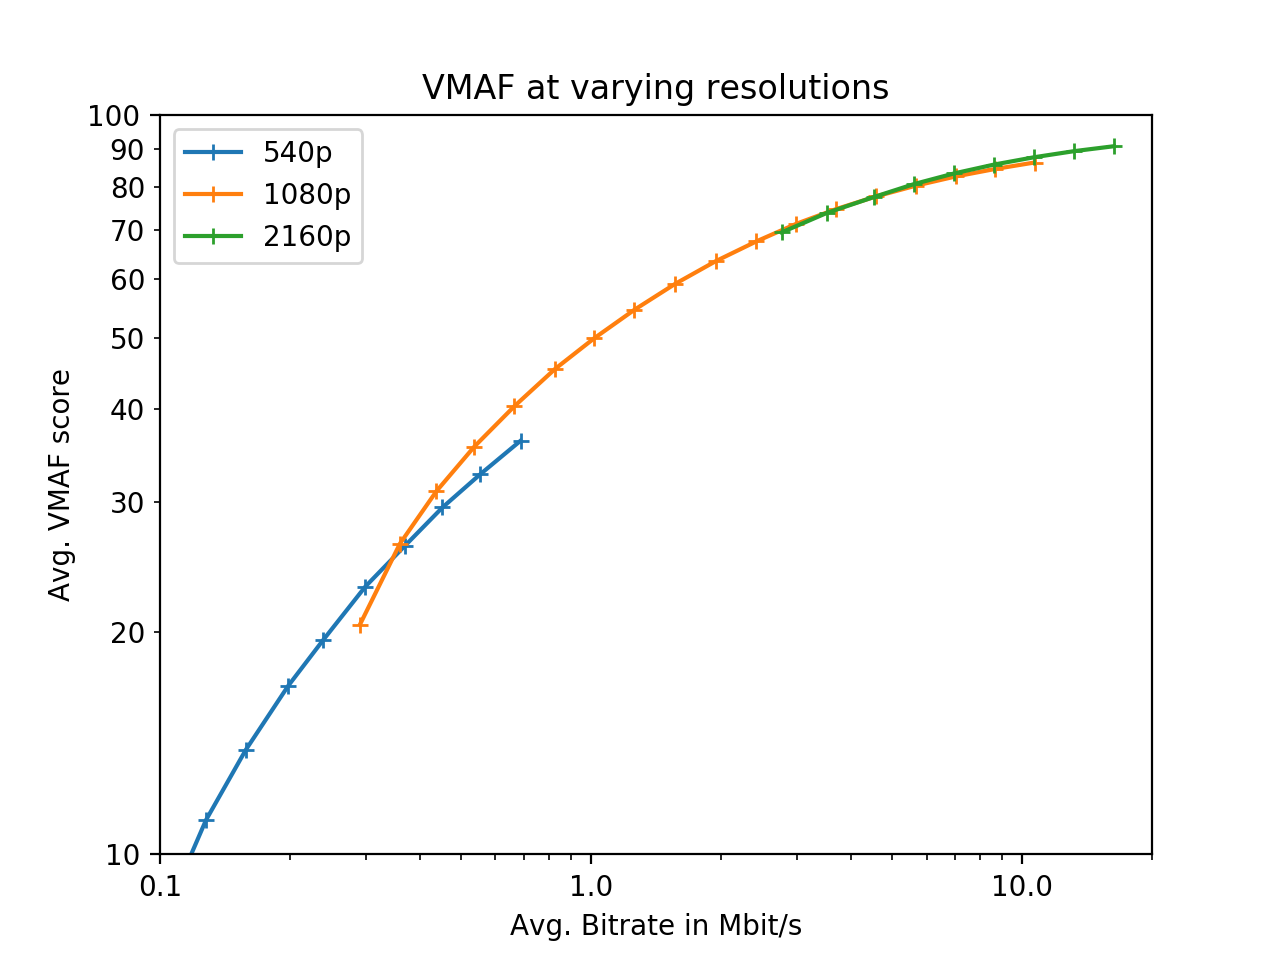
\includegraphics[width=3.5in]{vmaf_bitrates}
	\caption{VMAF scores for 25 different bitrates at 3 resolutions}
	\label{fig:vmaf:bitrates}
\end{figure}

\subsubsection{Encoding Presets}
Two different presets are used for the sequence encodings, a "na\"{\i}ve" and an "expert" preset. The  "na\"{\i}ve" preset is a simple CBR encoding, whereas the "expert" preset is a 2-pass encoding with a Q-CTRL pass followed by a B-CTRL pass.  Every sequence is encoded with both presets at 3 resolutions (540p, 1080p, 2160p) and 3 bitrates for each resolution. The resulting VMAF-scores for the encoded sequences can be seen in figure \ref{fig:vmaf:encoded}. The following section explains our method for the bitrate selection.

\subsubsection{Selection of Bitrates}
Video Multi-Method Assessment Fusion (VMAF) is a full reference metric for estimating human perception of video quality \cite{lin2014:fvqa}.

To estimate relevant HEVC bitrates for our source content we sample the VMAF scores at 25 bitrates on a logarithmic scale for our 3 different resolutions (540p, 1080p, 2160p). The reference sequences are resampled to a fixed 50 frames per seconds to avoid frame rate differences, while the distorted sequences are downsampled, encoded with CBR rate control and upsampled to UHD-1 again using lanczos resampling. Both presets use 4:2:0 chroma subsampling to be close to the typical use-case of webvideo. The resulting VMAF scores exhibit an overlap between different resolutions and the final encoding bitrates are chosen near those intersections. Figure \ref{fig:vmaf:bitrates} shows the sampled scores (foreground) and the target rates (background). The bitrates are chosen at least 2 bitrate-samples away from an intersection with the next quality, except for the lower 1080p-bound where this is not possible due to encoder restrictions, as is fails to encode for even lower bitrates.

\begin{figure}[!t]
	\centering
	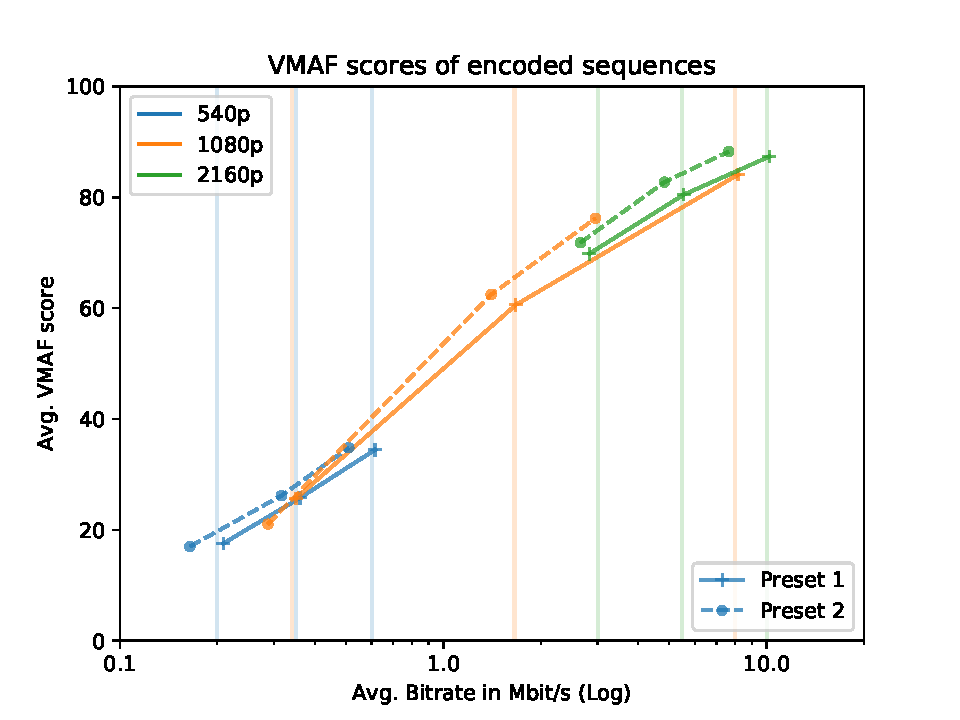
\includegraphics[width=3.5in]{vmaf_final}
	\caption{VMAF scores of encoded videos}
	\label{fig:vmaf:encoded}
\end{figure}

\begin{figure}[!t]
	\centering
	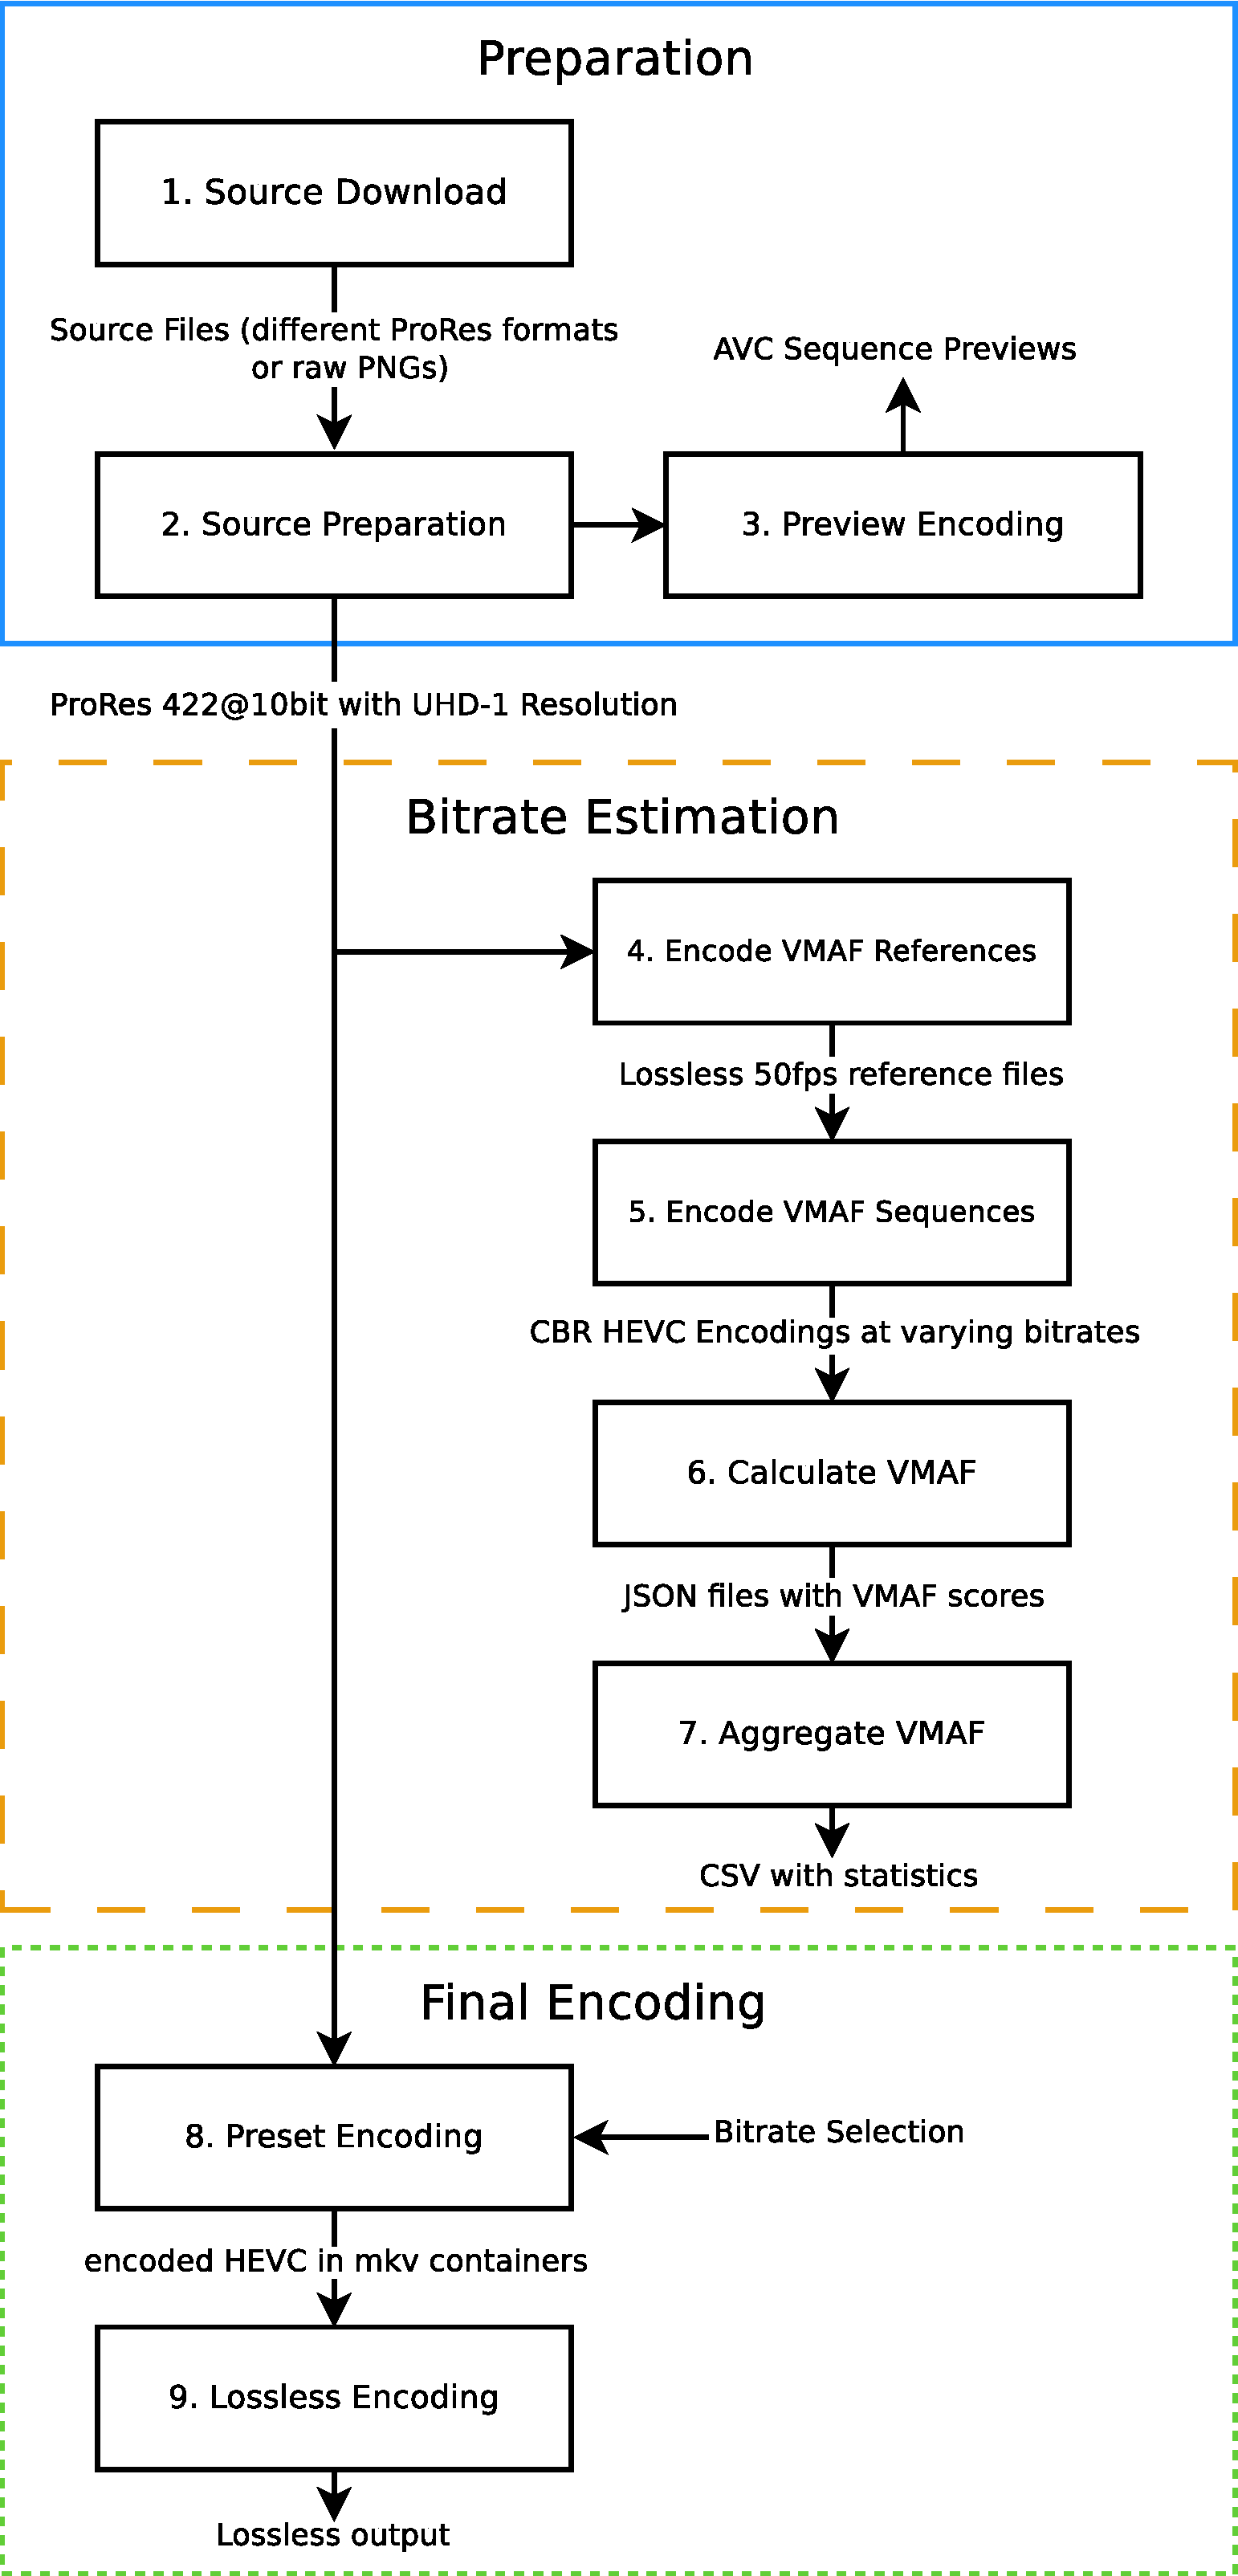
\includegraphics[width=3in]{automation}
	\caption{Automated processing and encoding workflow for providing }
	\label{fig:automation}
\end{figure}

\subsubsection{Encoding Automation}
We automate the whole process for downloading, preprocessing and encoding the source videos using pydoit \cite{web:pydoit}.

The process is illustrated in figure \ref{fig:automation} and starts with the source preparation (Blue box). After downloading the sequences (1) they are cut to 10 seconds length and saved as ProRes HQ with UHD-1 resolution (2). Additionally, h.264 previews are generated at a lower resolution of 1440p to allow reviewing of sequences on slower devices.

After the initial preprocessing videos are brought to an equal 50fps framerate (4) and encoded at different bitrates (5). The VMAF score of each video is analyzed.



